\documentclass[12pt,letterpaper]{article}
\usepackage{amsmath,amsthm,amsfonts,amssymb,amscd}
\usepackage{listings}
\usepackage{color}
\usepackage{MnSymbol,wasysym}
\usepackage{caption}
\usepackage{subcaption}

\definecolor{dkgreen}{rgb}{0,0.6,0}
\definecolor{gray}{rgb}{0.5,0.5,0.5}
\definecolor{mauve}{rgb}{0.58,0,0.82}

\lstset{%frame=tb,
  language=Bash,
  aboveskip=3mm,
  belowskip=3mm,
  showstringspaces=false,
  columns=flexible,
  basicstyle={\small\ttfamily},
  numbers=none,
  numberstyle=\tiny\color{gray},
  keywordstyle=\color{blue},
  commentstyle=\color{dkgreen},
  stringstyle=\color{mauve},
  breaklines=true,
  breakatwhitespace=true
  tabsize=3
}


\usepackage{hyperref}
\usepackage{graphicx}
\usepackage{enumerate}
\usepackage{fancyhdr}
\usepackage{mathrsfs}
\usepackage[margin=3cm]{geometry}
\setlength{\parindent}{0.0in}
\setlength{\parskip}{0.05in}

% Edit these as appropriate
\newcommand\course{CS595}
\newcommand\semester{Fall 2013}     
\newcommand\hwnum{7}
\newcommand\yourname{Mohamed Aturban}
\newcommand\login{maturban}

\newenvironment{answer}[1]{
  \subsubsection*{Problem #1}
}

\pagestyle{fancyplain}
\headheight 40pt
\lhead{\yourname\ (\login)\\\course\ --- \semester}
\chead{\textbf{\Large Assignment \hwnum}}
\rhead{\today}
\headsep 40pt

\begin{document}

All files mentioned in this document should be uploaded into the {\it github} repository.

\begin{answer}{1}

The same R script, {\it rcode.r} from assignment 6, has been modified to ,first, read data from \url{http://vlado.fmf.uni-lj.si/pub/networks/data/ucinet/zachary.dat}, and then create two {\it .json} files ({\it before.json} and {\it after.json}) which, respectively, describe the Karate Club graph before and after the split by Girvan-Newman algorithm. The following piece of code is for achieving the first task of reading data-- weighted edges from the above link and assigning this graph to a variable named {\it g}. 
\begin{lstlisting}
	  tmp <- getwd()
	  url <- "http://vlado.fmf.uni-lj.si/pub/networks/data/
	          UciNet/zachary.dat"
	  dest <- paste(tmp, sep="/", "k.dat")
	  download.file(url=url, destfile=dest)
	  l <- readLines(dest)
	  l <- l[(grep("^DATA", l)+1):length(l)]
	  l1 <- matrix(scan(textConnection(paste(l[1:34],
	        collapse="\n"))), nr=34)
	  l2 <- matrix(scan(textConnection(paste(l[1:34+34],
	        collapse="\n"))), nr=34)
	  karate_unweighted <- graph.adjacency(l1, weighted=TRUE,
	                       mode="undirected")
	  karate_weighted <- graph.adjacency(l2, weighted=TRUE,
	                       mode="undirected")
	  g <- karate_unweighted                       
\end{lstlisting}

While the following lines of code is to produce the two output files ({\it before.json} and {\it after.json}). The code is not too long( one page and a half), so it is shown below:
\begin{lstlisting}
# Create Edges vector Before split
original_vec <- numeric()
for (i in 1:ecount(g)) {
	for (j in 1:ecount(karate_weighted)) {
		s1 <- get.edgelist(g)[i,1]
		s2 <- get.edgelist(g)[i,2]
		d1 <- get.edgelist(karate_weighted)[j,1]
		d2 <- get.edgelist(karate_weighted)[j,2]
		if ((s1 == d1) && (s2 == d2))
		{
			original_vec <- append(original_vec,get.edgelist
                                         (karate_weighted)[j,1] - 1)
			original_vec <- append(original_vec,get.edgelist
                                         (karate_weighted)[j,2] - 1)
			original_vec <- append(original_vec,
                                         E(karate_weighted)$weight[j])
		}
	}
}
# Create Edges vector After split
vec <- numeric()
for (i in 1:ecount(g)) {
	for (j in 1:ecount(karate_weighted)) {
		s1 <- get.edgelist(g)[i,1]
		s2 <- get.edgelist(g)[i,2]
		d1 <- get.edgelist(karate_weighted)[j,1]
		d2 <- get.edgelist(karate_weighted)[j,2]
		if ((s1 == d1) && (s2 == d2))
		{
			vec <- append(vec,get.edgelist
                                         (karate_weighted)[j,1] - 1 )
			vec <- append(vec,get.edgelist
                                         (karate_weighted)[j,2] - 1 )
			vec <- append(vec,E(karate_weighted)$weight[j])
		}
	}
}

# Create Data Frames for Edges and nodes before and after split

# Edges before split
o <- matrix(original_vec,ncol=3,byrow = TRUE)
edgeBefore <- as.data.frame(o)
colnames(edgeBefore) <- c("source", "target","value")

# Edges after split
m <- matrix(vec,ncol=3,byrow = TRUE)
edgeAfter <- as.data.frame(m)
colnames(edgeAfter) <- c("source", "target","value")

# Nodes before split
c <- 1
a <- as.numeric( unlist(clusters(karate_unweighted)['membership']))
vecnode <- numeric()
for (i in 1:34) {
	vecnode <- append(vecnode,c)
	vecnode <- append(vecnode,a[i])
	c <- c + 1
}
matnode <- matrix(vecnode,ncol=2,byrow = TRUE)
nodeBefore <- as.data.frame(matnode)
colnames(nodeBefore) <- c("name","group")

# Nodes after split
c <- 1
a <- as.numeric( unlist(clusters(g)['membership']))
vecnode <- numeric()
for (i in 1:34) {
	vecnode <- append(vecnode,c)
	vecnode <- append(vecnode,a[i])
	c <- c + 1
}
matnode <- matrix(vecnode,ncol=2,byrow = TRUE)
nodeAfter <- as.data.frame(matnode)
colnames(nodeAfter) <- c("name","group")


# Create Output Files in JSON format
toJSONarray <- function(dtf){
	clnms <- colnames(dtf)
	name.value <- function(i){
		quote <- '';
		if(class(dtf[, i])!='numeric' && class(dtf[, i])!=
		'integer'){ 
			quote <- '';
		}
		paste('"', i, '" : ', quote, dtf[,i], quote, sep='')
	}
	objs <- apply(sapply(clnms, name.value), 1, function(x){paste(x,
	collapse=', ')})
	objs <- paste('{', objs, '}')
	res <- paste('[', paste(objs, collapse=',\n'), ']')
	return(res)
}

# JSON file before split
outputstr = paste('{\n"nodes":\n', toJSONarray(dataFramenodebefore))
outputstr = paste(outputstr, ',\n"links":\n')
outputstr = paste(outputstr, toJSONarray(dataFrame1))
outputstr = paste(outputstr, "\n}\n")
fileConn<-file("before.json")
writeLines(outputstr, fileConn)
close(fileConn)
# JSON file after split
outputstr = paste('{\n"nodes":\n', toJSONarray(dataFramenode))
outputstr = paste(outputstr, ',\n"links":\n')
outputstr = paste(outputstr, toJSONarray(dataFrame2))
outputstr = paste(outputstr, "\n}\n")
fileConn<-file("after.json")
writeLines(outputstr, fileConn)
close(fileConn)

                     
\end{lstlisting}


After, successfully, getting the two files ({\it before.json} and {\it after.json}) , it is time now to use {\it d3 js} to simulate the two graphs before and after the split. The following steps, briefly, describe how the code, in {\it index.html}, works:

\begin{itemize}
\item Read the graph vertices and edges from {\it before.json}
\item Draw its nodes, edges, and labels.
\item When clicking, by mouse, on any of the nodes (here, the click should not be on the node label), the current graph will be removed from the screen. Instead, vertices and edges from {\it after.json} will be drawn.
\item If you click , again, on any node within the two graphs, the same scenario will be repeated from step 1. 
\end{itemize}



{\bf Output samples:}


\begin{enumerate}

\item The code can be tested online at:

      \url{http://www.cs.odu.edu/~maturban/indexmoh.html}
 
\item Figure 1. shows the web-page when first loaded. It contains a green sentence which guides the user of how the graph(s) can be split/merged.


\begin{figure}[ht!]
\centering
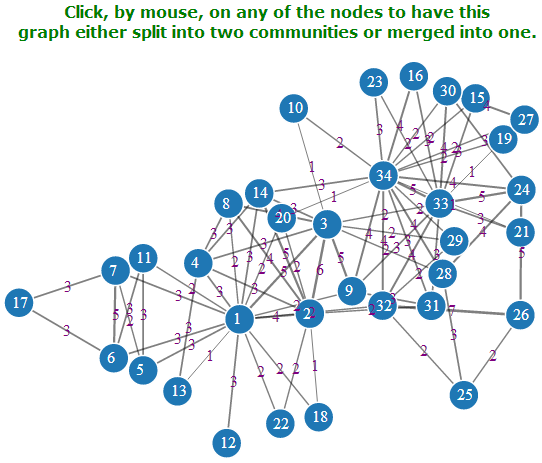
\includegraphics[scale=0.8]{graphone}
\caption{Karate Club graph before split}
\label{overflow}
\end{figure}
 

  \item Now, if clicking on any node, not on the node label, the graph will be split into two clusters as you can see in figure 2.

  \item By clicking again on any node within the two graphs, they will be merged into one graph as shown in figure 1.

\end{enumerate}

\begin{figure}[ht!]
\centering
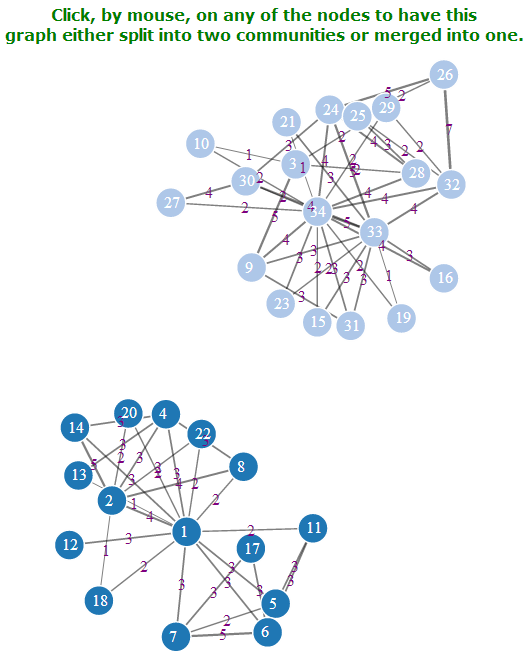
\includegraphics[scale=0.8]{graphtwo}
\caption{Karate Club graph after split}
\label{overflow}
\end{figure}


{\it index.html} is uploaded into the course repository. Also, I would like to mention that I uploaded the file {\it reference.txt} which contains all resources I have used for this assignment. As you suggested, starting from next assignment (no. 8), I will try to use BibTex for references (I promise).

\end{answer}

\begin{answer}{2}
I was interested to see my followers graph on Twitter using D3, but it is matter of time. 
\end{answer}

\end{document}
